\section*{Parallelization Steps}
\begin{description}
    \item[Sequential Program]Sequential Steps + Programming (Application specification $\rightarrow$ executable program)
    \item[Parallel Program]Parallelization + Programming. \\ %Analysis of seq. problems or programs to identify parallelism. \\
        % 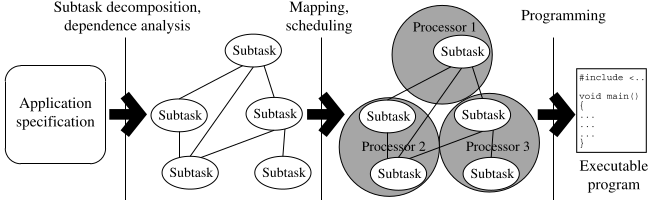
\includegraphics[width=0.4\linewidth]{paralellization.png} %TODO: modify image to include TLB
        \item[Decomposition] of apps into functional tasks / data blocks. (expose inherent concurrency). \textbf{Types:} \textbf{Data} exploits data parallelism, \textbf{Functional} expl. funct. parallelism. \textbf{Recursive} divide and conquer (exploits d or f). \textbf{Explorators} search problems, exp. data p. \textbf{Speculatory} exploit and employ if-statements. ex. f. dec. \\
        \textbf{Influencing Factors:}
        \begin{itemize}
            \item \textbf{Application Type}: distinct steps or iterative block of computations (task parallel, data parallel) %TODO: task parallel und data parallel erklären
            \item \textbf{Concurrency degree (max, avg)}: depending of degree of inherent parallelism. all/enough or none can be executed concurrently.
            \item \textbf{Granularity}: computational size of tasks / data blocks after decomposition. (fine, medium, coarse)
            \item \textbf{Target system}: affects costs of synchronization and communication. (\textit{Shared-mem arch}: support fine-grain decomp. inexpensive more frequent s \& c, \textit{Distr. mem arch}: usually require coarse-grain decomp. more expensive and less frequent.)
        \end{itemize} %TODO: look at examples S. 20-23
    \item[Dependence Analysis]is critical to identify how much parallelism exists \& how it can be exploited. Types of Dependencies:
        \begin{itemize}
            \item \textbf{Control}: describe control structure of f. dec. application. Impose precedence order on execution of tasks.
            \item \textbf{Data}: describe data transfers (d. dec. application). \textit{flow (true) deps}: one task writes, another reads $\rightarrow$ also results in prec. order.
            \item \textbf{Name}: 2 tasks use same register/mem location without any data flow. (no true deps) \textit{Anti-Deps}: one task reads, another writes. \textit{Output deps}: both tasks write same var.
        \end{itemize}
        \item[Mapping] (assignment, part of scheduling) the exectuion of tasks / operations on data onto computing system.
        \begin{itemize}
            \item \textbf{Spatial assignment}: placing subtasks onto processing elements. (Where will a subtask be executed)?
            \item \textbf{Temporal ordering}: assign start time to subtask (When)?
            \item \textbf{Static/Dynamic Mapping}: offline (before exec.), online (during exec.). (How is a subtasks mapping performed)?
        \end{itemize}
        \item[Programming] or expressing parallelism in programming language.
        % TODO: S. 30 Models and Paradigms for Programming (Shared Memory with Threads)
        \item[] Note: Performance now a programmers charge. (cannot rely on HW anymore).
\end{description}
\section*{Parallel Programming}
\begin{description}
    \item[How?] Extend Compilers, \textbf{Extend languages}, Stack languages or New language \& Compiler Set
    \item[Pros] easiest, quickest, cheapest (effort, time). leverages existing compiler tech, new libs ready fast.
    \item[Cons] lack of compiler support to catch errors (P creation, term., sync and communication), easy to write "bad" programs
    % \item[Standards: Shared-Memory Approach with OpenMP] TODO:
    \item[Parallel Multithreaded Programming]Multiple Ts (independent flow of control within one P with its own context (stack \& register set)). shares P data and opened files. Lower overhead. %TODO: S. 35
\end{description}
\subsection*{OpenMP}
API for writing Multithreaded Applications: Compiler Directives, Library Routines. for C/C++ and Fortran. Standardizes SMP (symmetric multiprocessing). #include "omp.h"
\begin{description}
    \item[Pros] Widely available on many multicore computers, works OS-independent, fewer code modifications than using message passing, directives are treated as comments when OpenMP not available, directives can be added incrementally.
    \item[Cons] Doesn't run on distributed memory computers, requires compiler which supports OpenMP, limited by #cores available, may have lower parallel efficency.
    \item[Components]\textbf{Directives (Pragmas)}, \textbf{Runtime Lib routines}, \textbf{Env. variables} %TODO: diagrams S. 39, 40
    \begin{itemize}
    \item \textbf{Structured Blocks}: between \{\}. \textbf{Conditional Compilation} #ifdef \_OPENMP... \textbf{Continued lines} with \textbackslash
        \item \textbf{Parallel regions (D)} fork when encountering parallel region (worker thread team/pool started). implicit join. sleep until needed again.
        \item \textbf{Work Sharing (D)}: OpenMP designed for parallelize loops (for-loops). \textit{\#pragma omp parallel for} splits loops between multiple threads. With \textit{\#pragma omp parallel} each thread executes each loop iteration.
        \item \textbf{Runtime Library (RTL) functions}: functions executed during runtime
    \end{itemize}
\end{description}
